% 	Benjamin Van Durme, vandurme@cs.rochester.edu, 24 Aug 2009
%
% Purpose: an example .tex file for the thesis.
%
% This file was derived from those used by Ashwin Lall and Piotr Faliszewski in
% their respective thesis works.

\documentclass[11pt,leqno]{report}

% Feb 24, 2010 vandurme> I used a separate header.tex to capture personal
% shortcuts, and included packages. This allowed my to create mini-documents
% based on each chapter, by having a distinct top-level file around each of the
% files "\include"-ed below, that could each then use the same header (so
% changes would be kept in sync):
%
%\input{header}
%
% The first two things in that header:
%\usepackage{urcsbiblio}
%\usepackage{urcsthesis}

\pdfinfo{
/Title (Extracting Implicit Knowledge from Text)
/Author (Benjamin D. Van Durme)
/Keywords (thesis, knowledge acquisition, information extraction)
}

\begin{document}

\sloppy
\title{Extracting Implicit Knowledge from Text}
\author{Benjamin D. Van Durme}
%\thesissupervisor{Professor Lenhart K. Schubert}
\maketitle

% Feb 24, 2010 vandurme> the graduate office wanted a "ii" on the top right
% corner of the dedication page (lowercase Roman numeral page numbering), which
% explains the slightly messy tex code for this page:

%%%dedication page
\thispagestyle{empty}
%\thispagestyle{plain}
\newenvironment{dedication}
{\cleardoublepage \thispagestyle{empty} \vspace*{\stretch{1}}
  \begin{center} \em}
  {\end{center} \vspace*{\stretch{3}} }
\begin{dedication}

  %% To ... 

\end{dedication}

%%% CV page
%\begin{curriculumvitae}

  Benjamin David Van Durme was born in Dansville, New York on November~13th,
  1979. He began studies at the University of Rochester in 1997, graduating in
  2001 with a Bachelor of Arts degree in the area of Cognitive Science and a
  Bachelor of Science degree in the area of Computer Science. From 2002 to 2004,
  he attended Carnegie Mellon University, and graduated with a Master of Science
  degree in Language Technologies. Benjamin returned to the University of
  Rochester in the Fall of 2004, pursuing research in the subjects of Computer
  Science and Linguistics, under the direction of Professor Lenhart K. Schubert.
  He received the Master of Science degree in Computer Science from the
  University of Rochester in 2006. During the Summer of 2006, as well as 2007,
  Benjamin performed research at Google Inc., under the direction of Marius
  Pa\c{s}ca.

\end{curriculumvitae}

\begin{acknowledgments}

  To my committee as a whole, William Cohen, Gregory Carlson, Daniel Gildea, and
  Lenhart K. Schubert: thank you for your advice and guidance.

  %% Additional personal acknowledgments ...

  Chapter~\ref{ch:Framework} is the result of extensive discussions with Len
  Schubert on a variety of semantic phenomena. Chapter~\ref{ch:Methodology}
  derives from joint work with Len Schubert \cite{vandurmeSTEP08}.
  Chapter~\ref{ch:UsingClasses} is the result of joint work with Ting Qian and
  Len Schubert \cite{vandurmeCOLING08}. Material from
  Chapter~\ref{ch:LearningClasses} is based on collaboration with Marius
  Pa\c{s}ca while at Google Inc. \cite{vandurmeAAAI08}.
  Chapter~\ref{ch:UsingOntology} is based on joint work with Phillip Michalak
  and Len Schubert \cite{vandurmeEACL09}. Chapter~\ref{ch:TopicModels} is based
  on work performed with Dan Gildea \cite{vandurmeTR09}.

  This material is based upon research supported by National Science Foundations
  awards, IIS-0328849 entitled ``Deriving General World Knowledge from Texts by
  Abstraction of Logical Forms'', IIS-0535105 entitled ``Knowledge
  Representation and Reasoning Mechanisms for Explicitly Self-Aware
  Communicative Agents'' and CCF--0910415 entitled ``RI: Small: General
  Knowledge Bootstrapping from Text'', in addition to a University of Rochester
  Provost's Multidisciplinary Award (2008), entitled ``Computational
  Psycholinguistics: Integrating Computational and Behavioral Methods to Study
  Human Language Processing''. Any opinions, findings, and conclusions or
  recommendations expressed in this material are those of the author and do not
  necessarily reflect the views of above named organizations.

\end{acknowledgments}

\begin{abstract}

  The everyday intelligence of both humans and machines relies on a large store
  of background, or common-sense, knowledge. That such a knowledge base is not
  yet available to machines helps partially explain the community's inability to
  provide society with the sort of synthetic intelligence described by futurists
  such as Turing, or Asimov.

  In response, there have emerged a variety of methods for automated
  \emph{Knowledge Acquisition (KA)} that are now being actively explored. Here I
  consider the extraction of knowledge that is conveyed \emph{implicitly}, both
  within everyday texts and queries posed to internet search engines. Through
  recognizing certain forms of existential predicative patterns, and abstracting
  from these to more strongly quantifiable statements, I show that a significant
  amount of general knowledge can be gleaned based on how we talk about the
  world. I provide experimental results both for the direct extraction and
  strengthening of such knowledge, and for the automatic acquisition of
  supporting resources for this task.

  In addition, I draw attention to the relationship between automatically
  acquired background knowledge and natural language \emph{generic} sentences.
  Humans use generics when they wish to directly assert the same sorts of
  ``rules of the world'' that are of concern to the KA community. And yet, there
  has been little recognition in applied circles that decades of work from
  formal linguistic semantics may have a role to play in the representation, and
  perhaps even the acquisition, of common knowledge.
  
\end{abstract}

\tableofcontents
\listoftables
\listoffigures

%Introduction
Crowdsourcing has shown to be an effective means of solving tasks that are computationally difficult, or otherwise impractical, for artificial intelligence programs to solve. \cite{howie2006rise}. 
There are many instances, of course,where humans are more effective than machines and vice-versa. 
To pick the most obvious example: humans are more efficient at qualitative, ambiguous tasks, while artificial intelligence (AI) agents tend to be better at more quantitative, direct tasks.
Naturally, most tasks do not fall cleanly into one category or another; there are many tasks which cannot be done perfectly by human or AI agents. 
For this reason, the merging of human and AI is necessary for the completion of a number of tasks.

Consider, for example, the task of building an instruction manual for a common profession. 
If a restaurant wanted to create a manual for a number of everyday tasks in the restaurant in order to train new employees quickly.

ADD SOMETHING ABOUT THIS BEING ABOUT SKILLED USERS

It would use data gathered from existing employees to solve this task, as the ambiguous and qualitative data of procedural tasks such making food and settling tables is far beyond the current capabilities of artificial intelligence.
One experienced employee could be delegated to the task-instruction creation, but there are a number of issues with this method.
First, an over-reliance on one individual leaves the system vulnerable to error.
An individual may make mistakes when writing instructions.
The only solution to this problem would be to have other users check the first users work, which automatically means that multiple users will be needed regardless.
Second, many task, especially the qualitative, ambiguous ones previously mentioned, can be done in multiple ways.
While the differences may not necessarily be erroneous in nature, they can pose problems.
Certain delis, for example, have managers with different policies on the quality of meat used for sandwiches.
If a trainee is taught the preference of one manager and not the other, issues can arise if the employee switches managers.
Third, there are many instances where individuals have been shown to be slower than crowds \cite{lasecki2013interactive,}.
It it likely that crowd-sourced users will also be more efficient than single users in this domain.

One major issue with gathering instructions from users is dealing with redundancy.
Because many people have similar notions of instructions for various tasks, users tend to give similar instructions for a given step.
This leads to redundancy. For example, if a group of 3 users were asked to write the first step for making a peanut-butter and jelly sandwich, the users might respond with
\begin{enumerate}
\item get two slices of bread
\item get two slices of bread, a knife, peanut butter, and some jelly
\item get the ingredients.
\end{enumerate}
It is obvious in this situation that because suggestion 3 is described completely (and more thoroughly) by suggestion 2, that it is redundant and thus can be removed.

Failure to do so can impede the crowd-sourcing process.
First, it introduces a form of noise into the system.
With multiple identical sentences, if users are asked to vote on the suggestions, the voting process may be subverted.
Consider the same situation as the last example, but the three inputs are
\begin{enumerate}
\item get two slices of bread
\item get the ingredients
\item get the ingredients.
\end{enumerate}
If two users believe that option 2 (or equivalently, option 3) is correct, they could vote for either. 
If the third user votes for option 1, then there is no clear majority from voting, even though the consensus is clear.

This problem ultimately is an issue of natural language processing, and is unique in that it deals with very short documents in a very small corpus. 
A quick and efficient method of removing and/or minimizing redundancies in the context of this problem is essential to the completion of the task.

In total, the task of building a set of instructions (or a ``how-to'' manual) efficiently from a group of users requires efficient crowd-sourcing techniques as well as sufficiently sophisticated AI to augment this process.
Although there has been much research on using crowds to answer single questions, there has not been much work done in the next level of abstraction: having users answer lists of questions (i.e. instructions) \cite{lasecki2013chorus,bigham2010vizwiz}.

The remainder of this paper will be organized as follows:
\begin{itemize}
	\item the Background section will discuss previous work done in both crowdsourcing and redundant sentence removal, as well the unresearched areas where this project will make its contributions
	
	\item The Methodology section will describe the Canned Mentorship system in detail, both at an algorithmic and implementation level. It will also descirbe the parameters tested and the experimental setups.
	
	\item The results section will describe the experimental results of the study, and discuss the any anomalies or other observations encountered during the testing process.
\end{itemize}

%background

\section{Crowdsourcing}
Crowdsourcing has shown itself to be a very effective computational resource.
Formally, it is defined as
\begin{quote}
the act of a company or institution taking a function once performed by employees and outsourcing it to an undefined (and generally large) network of people in the form of an open call. \cite{brabham2008crowdsourcing}.
\end{quote}

\subsection{Current Scope and Usage of Crowdsourcing}
Though crowdsourcing covers a very broad range of activities and fields, it is possible to define separate catagories. Brabham defined three separate categories:
\begin{enumerate}
	\item crowdfunding
	\item crowd labor 
	\item crowd research.
\end{enumerate} 

Crowdfunding is the use of crowd-based resources to fund projects. Websites such as gofundme.com, kickstarter, and patreon.com are all crowdfunding website which allow elicit funds from users. 
This method is particularly useful for freelance artists \cite{brabham2008crowdsourcing}.

Crowd labor utilizes the crowd for computation and other work-like tasks. Generally, this involves the users doing low effort tasks for low pay. 
In many situations, this can result in a much cheaper product than non crowdsourced, professional settings.

For example, the stock photo website iStockphoto collects images uploaded by users, and pays them a small compensation for their effort. This website is able to lease the rights to these images for \$1, which undercuts professional photographers' prices by over $90\%$ \cite{howe2006rise}.



% tips for crowd motivaiton: 4 f's fun, fulfillment, fame, fortune
%crowdsourcing
%crowd sourcing in general

%redundant sentence removal
%sentence comparisons
%semantic distance between sentences
%hierarchical clusting of sentences
%unsupervised learning of setnences
       
                         
\include{framework}        

The efficacy of the program was dependent on its ability to coordinate users and ensure that they were able to work together to generate the final instructions.
Thus, it was necessary to not only design an effective workflow, but to also make sure that the program implementation was easy to understand, robust, and close to the theoretical workflow.

\section{Workflow}
Turkomatic ran into difficulties in organizing the workflow. 
Their system was unable to coordinate workflows, in no small part due to the complexity of the algorithm.
Their algorithm used recursive workflow partitioning, and allowed for complex sub-task creation.
This led to significant difference of opinion between users, and little consensus was obtained without the use of a single task evaluator who would oversee the task.
\todo{todo: describe more thorougly the turkomatics issues with task division}.

\subsection{Greedy Instruction Addition}
Taking the opposite mentality, CannedMentorship uses a very simple task generating algorithm, with no explicit task subdivision or branching.
The system simply asks users to create steps in sequence, from beginning to end, in order.
Each step is completed in order, with the latter steps coming directly after former steps chronologically. 

\section{Implementation and Webapp details}
Our project began by creating a small webapp which coordinated the instruction generating process.
This program, also dubbed ``Canned Mentorship,'' consisted of two separate programs:

\begin{enumerate}
	\item a website interface for coordinating working users
	\item a back-end AI script for classifying answers and removing redundant inputs
\end{enumerate}

\section{System Implementation}

\subsection{The Webapp}
The webapp was a program written using Python Flask and was hosted on Heroku webapps. 
It was designed as a lightweight, simple system which hosted the users for the duration of the task and also coordinated their actions.

\begin{figure}[h]
	\begin{center}
		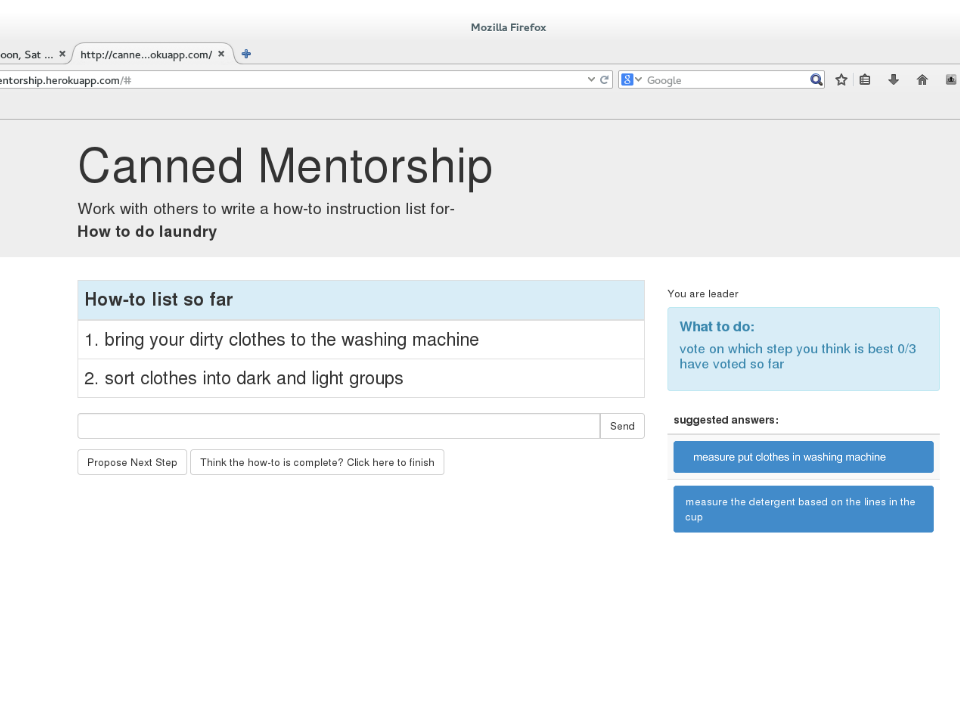
\includegraphics[width=0.48\textwidth]{figures/cmInterface2.png}
		\caption{Rejection sampling was also considered as a placement mechanism.}
		\label{fig:rejection_sampling_placement}
	\end{center}
\end{figure}

As noted earlier, Heroku was chosen as the host location for the webapp ...add more stuff later...



%webapp description
%theory
%workflow
%implementation

%ai backend
%interface with program
%parameters
	%reasons for choosing
%flow
%
\begin{comment}
\begin{figure}[h]
	\begin{center}
		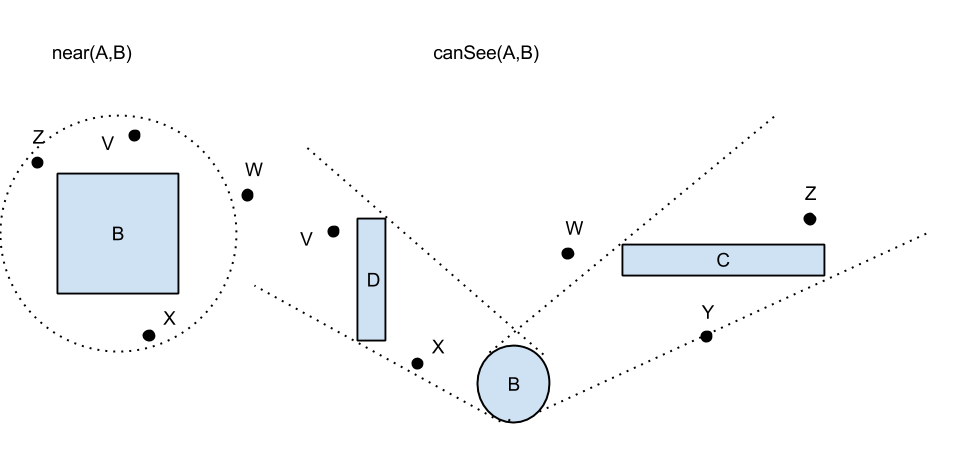
\includegraphics[width=0.48\textwidth]{figures/rejection_sampling_placement.png}
	\caption{Rejection sampling was also considered as a placement mechanism.}
	\label{fig:rejection_sampling_placement}
	\end{center}
\end{figure}
\end{comment}      

\include{using-classes}    

\include{learning-classes} 

\include{using-ontology}   

\include{topic-models}     

As shown in figure the system is able to handle the simple case for object querying very reasonably. 
The fastest calculating predicate is \texttt{isTouching}, followed closely by \texttt{near}.
Because these two predicates operate on similar algorithms, it make sense that the two operate in similar time.
One potential significance is the fact that \texttt{isTouching} operates faster than \texttt{near}, and the only tangible difference between the two algorithms is the fact that \texttt{isTouching} has a smaller threshold than \texttt{near}.
It was first speculated that this meant that the internal Blender functions relied on by these predication functions' run-time increased with object distance.
However, the more likely explanation is the calculation of the threshold between the two functions.
In \texttt{near}, the threshold is calculated with a function that operates in linear time.
In \texttt{isTouching}, it is a constant, predetermined value, and thus requires no overhead to calculate.

The program worked into the Cornell Cup's Haptek team, where it was used to simulate a person navigating a virtual maze.  
This project set out to equip a room with several Kinect cameras which monitored the movement of a person in the room. A program, receiving input from the cameras, would build a virtual maze in a virtual representation of the room. The person's virtual avatar would be inserted into this simulation. 

The person's motion would be tracked with the cameras, and the avatar would move with the user. If the avatar came into contact with one of the virtual walls in the maze, then a buzzing feedback mechanism would be triggered. This allows the user to navigate a virtual maze. Because this is a simulation in 3D space, the project utilized many of the aspects of the \TDS project, including several of the predicates, the models for ``person'' and ``wall,'' and the temporal updating feature of the 3D scene.

In a similar note, the use of Blender has opened up a number of options for future endeavors. Because Blender is a widely-used program with a broad range of applications and widespread compatibility, \TDS has the potential to be utilized in any number of studies and situations. For example, many 3D printers currently accept model input in file formats supported by Blender. At this year's Rochack Hackathon, we were able to 3D print one of the models. This model can be seen in figure \ref{fig:3D_Print}.


The Blender file for the person was uploaded with minimal changes to the 3D printer at the school, and printed. The entire process of converting the file, uploading it to the printer, and printing the figure took less than an hour. Given the growing importance of 3D printing in the present, and the many applications to 3D environments that \TDS offers, the ability to quickly model objects that can be 3D printed could prove to be a valuable feature of the system.

An area of concern is the run-time of the ``inside'' predication.
The run-time of this predication is significantly worse than the others. Because this function runs in $O(n^2)$ time, it is most likely not due to an inefficient algorithm. Rather, this lack of satisfiability is likely related to the legal placement area generated by the placement function in predMethods.py.

Inside is similar to in, differing only in that it requires one object to be inside the mesh (rather than bounding box) of the other. The legal area, however, is generated to encompass the entire bounding box. As such, it may overestimates the legal area by a considerable amount. Shrinking the placement area would potentially solve this problem, though it may prevent placement in legal areas. 

Our project was able to successfully query and place entities under predicate constraints. Because the scene was able to pass the original test of constructing the story-based image and deduce the implicit, spatial information in the scene (the person could not see the egg in the nest), the study was a success. The efficacy of rejection sampling in the placement function requires further investigation. Current testing indicates that it improves scene construction by making placements more accurate, though the key issue in this endeavor is the efficiency of the inside predicate.

The placement system creates a complex relationship between predications and entities during placement. An ``optimal'' order of placement emerges in complex scenes. Deviation from the optimal layout was shown to increase placement time dramatically.

The ``optimal'' configuration is one in which the entities are placed in order of decreasing number of predication constraints. For example, in the placement of the story scene, the required predications are:
\begin{center}
	\begin{itemize}
		\item a person is under a tree
		\item a nest is in a tree
		\item an egg is in the nest
		\item the person can see the nest
	\end{itemize}
\end{center} 
In this scene, the nest is the most constrained object, because it is used in a predication with the person (can see), the egg (in), and the tree (in). The least constrained entities are the tree and the person, each involved in only one predication. This forms a ``constraint hierarchy.'' 

For an optimal placement run-time, the entities in the scene should be placed from the most to least constrained. Placing the most constrained entities first allows the most legal placement area for the subsequent entities (which, because they are lower in the hierarchy, have naturally less constrained placement areas), which means that the system has to do less sampling and backtracking on average in order to place them.
Note that a constraint hierarchy is not necessarily unique for a given scene because multiple entities can be involved in the same number of predications.

The greatest flaw in the system, and the biggest boundary to continued expansion of the project, is the ad-hoc nature of the predicate and object database. 
Both entities and predicates are created in an ad-hoc fashion; there exist no templates for either, although some share similar features. 
Because of this, adding new members to either library can be cumbersome. 
Further, because the predicate functions of each are based on qualitative semantic interpretations of the predicates, it can be quite difficult to write functions that objectively represent the predicates they are meant to.

Our project's success in creating and querying 3D scenes demonstrates both its usability as a situation for reasoning in 3D spaces, and the expressive power of the system in general. 
Our program was able to quickly and efficiently manage and query over a small library of entities and predicates. 
The system is black-boxed to outside input, and as such can be used for more than just Epilog. Preliminary work with the 3D printed model and the collaboration with Haptek has shown this. The system, in its current form, holds potential to be of use in a number of projects and experiments that involve 3D space. We hope that the \TDS will be put to use as a specialist program, both in Epilog and beyond.

\bibliographystyle{named}
\bibliography{references}

\appendix
\include{generics}


\end{document}



